\section{Słowem wstępu}
Każdy z nas zapewne staje często przed problemem kopiowania dużej ilości danych, czy to z nośników wymiennych, czy też z drugiego komputera. Czasami jednak jest to kopiowanie zaledwie kilku nowych, bądź zmienionych, plików, tak jak to ma miejsce podczas tworzenia kopii bezpieczeństwa. Nie ma wtedy sensu powielanie całych katalogów, a jedynie tych plików, które są zmodyfikowane lub nie znajdują się na naszych stacjach. Z pomocą przychodzą nam liczne programy, stworzone specjalnie, by ułatwić i zautomatyzować tą żmudną pracę. 

Programy do synchronizacji plików to narzędzia, które automatycznie kopiują, przenoszą, nadpisują i usuwają pliki pomiędzy wybranymi folderami. Jest to bardzo przydatna opcja, gdy korzystamy z kilku komputerów, a na każdym z nich chcemy mieć aktualne wersje danych. Synchronizacja polega więc na uaktualnieniu plików we wskazanych folderach do najnowszych dostępnych wersji oraz na selekcji jedynie tych, które takiej aktualizacji wymagają, co znacznie przyspiesza ten proces (więcej w przykładzie w rozdziale \ref{przyklad_lokal}). Co więcej, możliwa jest ona w obie strony, także po szyfrowanym kanale.

\subsection{Założenia projektu}
Celem mojego projektu było zaprojektowanie i oprogramowanie systemu do synchronizacji plików pomiędzy wieloma komputerami. W pierwszej jego części należało wykonać przegląd istniejących rozwiązań zarówno komercyjnych jak i darmowych. Zadaniem praktycznym było oprogramowanie systemu synchronizacji przy użyciu programu rsync lub pokrewnego.

Zadanie polegało na napisaniu odpowiednich plików wsadowych ,,.bat'', które ,,jednym kliknięciem''  pozwolą na synchronizację dowolnych katalogów i plików. Ważny jest tu dokładny opis parametrów skryptu, aby ułatwić konfigurację danych do synchronizacji, lokalizacji i adresu serwera. Dokładna instrukcja tworzenia tych plików oraz działania, znajduje się w rozdziale \\*\ref{skrypty}.

\section{Programy do synchronizacji}
\label{dosynch}
Wśród długiej i ciągle rozrastającej się listy oprogramowania do synchronizacji, znaleźć możemy pakiety, które składają się z serwera i klienta, korzystają z internetowego wirtualnego dysku, bądź posiadające program kliencki, do łączenia się z Linuxowym serwerem RSYNC.

\subsection{Pakiety serwer/klient}
Lista ta jest bardzo obszerna, jednakże postanowiłem zainstalować i przetestować kilka z nich.

\subsubsection{Allway Sync}
Uwagę moją przykuł darmowy \verb|Allway Sync| \cite{1}, który posiada bardzo intuicyjną obsługę (chociażby dzięki polskiej nakładce oraz licznym podpowiedziom), działanie na więcej niż jednym katalogu, synchronizację po sieci lokalnej i internetowej oraz z wymiennym dyskiem (patrz rys. \ref{allway}) oraz, jako jeden z niewielu, umożliwiał instalację na pendrive{}'ie lub zewnętrznym dysku twardym (wersja \verb|Allway Sync 'n' Go|) i posiadał dość rozbudowaną opcję automatycznej synchronizacji: przy starcie programu, po podłączeniu urządzenia, wykryciu zmian w folderach, co określony czas i oczywiście o podanej godzinie.
\begin{figure}[h!]
	\centering
	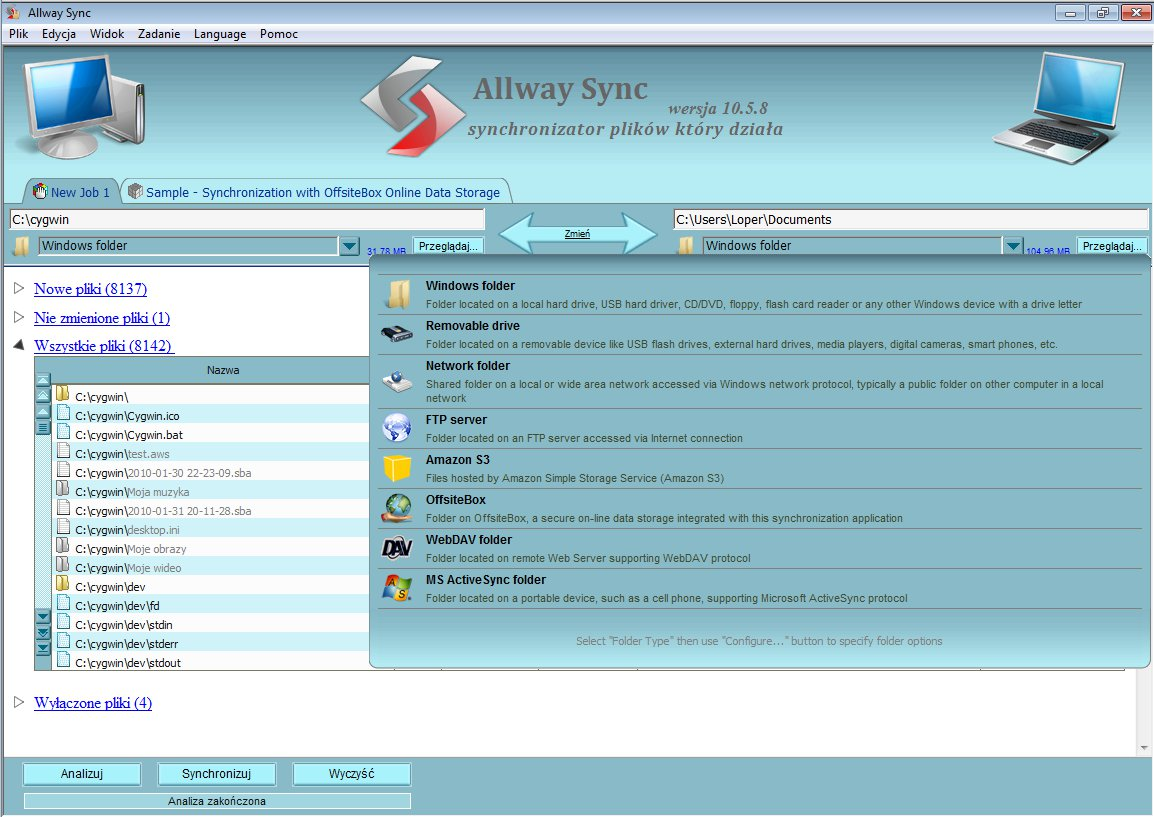
\includegraphics[width=1\textwidth]{img/s3.jpeg}
	\caption{Allway Sync - okno główne programu z listą źródeł synchronizacji}
	\label{allway}
\end{figure}

\subsubsection{GoodSync}
Godny uwagi jest także \verb|GoodSync| firmy \verb|Siber Systems| \cite{2} - również darmowy (oczywiście istnieje jego płatna wersja, oferująca więcej niż 3 zaplanowane zadania po 100 plików w każdym z nich). Oprócz podstawowych opcji, obecnych w każdym z testowanych przeze mnie programów, wyróżniał się bardzo dobrą analizą zależności między zadaniami (zmiany w jednym z nich, powodują natychmiastową reakcję w innym zadaniu, posiadającym te same ustalone foldery, a na przykład inną lokalizację docelową), kopiowanie po SMB, FTP, WebDAV i SSH, szyfrowanie i kompresję kopii, przejrzysty interfejs (patrz rys. \ref{goodsync}), dobrą automatyzację zadań (choć tu nie zadziała mi opcja synchronizacji przez FTP po wykryciu połączenia z internetem). Program również dostępny w polskiej wersji językowej.
\begin{figure}[h!]
	\centering
	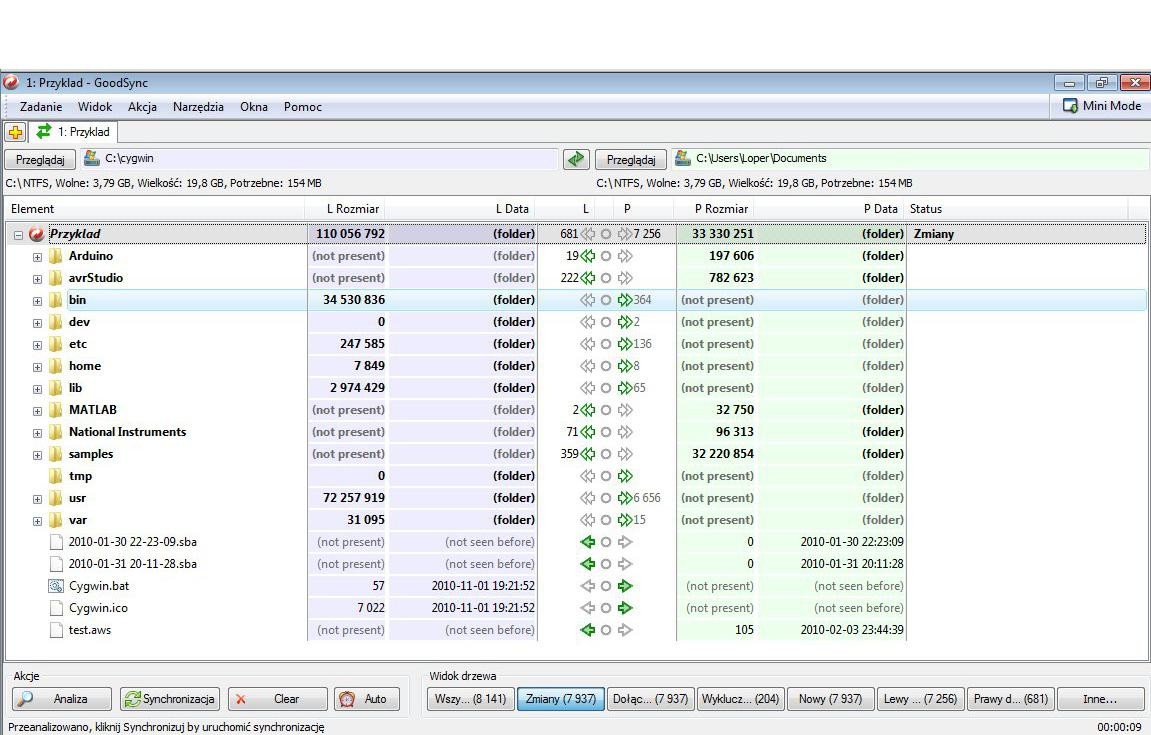
\includegraphics[width=1\textwidth]{img/s2.jpeg}
	\caption{GoodSync - przykład porównywania zawartości folderów}
	\label{goodsync}
\end{figure}

\subsection{Dysk wirtualny}
W tej kategorii warto wspomnieć o \verb|PowerFolder Basic| \cite{3} (patrz rys. \ref{power}). Jest to wieloplatformowa aplikacja napisana w języku Java. Posiada bardzo wygodną możliwość zarządzania, dostępnego z poziomu przeglądarki oraz moduł, który działa jako systemowy proces i monitoruje wszelkie zmiany. Producent oferuje 1GB dysk wirtualny (obecnie na okres 371 dni od rejestracji), również dostępny przez przeglądarkę. Ciekawą opcją jest wykonywanie (plików ,,.bat'') po zakończonej synchronizacji, dobrą kompresję danych ,,w locie'', bezpieczne przesyłanie danych (HTTPS, WebDAV przez SSL), ochronę przed przypadkowym usuwaniem plików, sumy kontrolne i wznawianie przerwanych transferów.\\
Minusem jest tu konieczność posiadania w miarę szybkiego łącza i plików o małych rozmiarach, w przeciwnym wypadku kopiowanie może trwać bardzo długo.
\begin{figure}[h!]
	\centering
	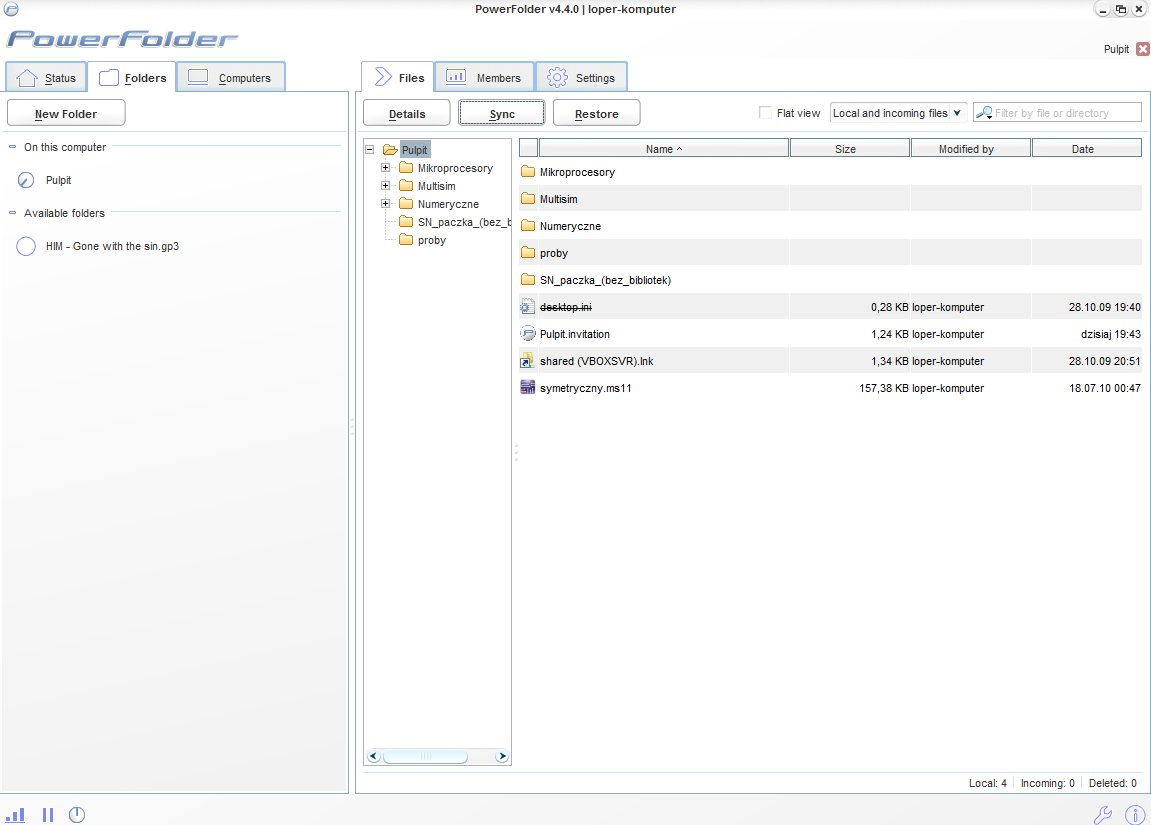
\includegraphics[width=1\textwidth]{img/s5.jpeg}
	\caption{PowerFolder - przesyłanie na wirtualny dysk}
	\label{power}
\end{figure}
\subsection{Kompatybilne z rsyncd}
Niestety, większość aplikacji nie posiada możliwości łączenia się z usługą \verb|rsyncd| (nasłuchującą standardowo na porcie 873). Jedynym programem umożliwiającym synchronizację kompatybilną z rsync, jaki udało mi się znaleźć, jest 
\verb|cwRsync| \cite{4}. Jako, że założeniem mojego projektu indywidualnego (opisanym na wstępie) było stworzenie systemu synchronizacji katalogów i plików pomiędzy klientem na systemie Microsoft Windows a serwerem rsyncd na systemie Linux, będzie to idealne rozwiązanie do wykonania, postawionego przeze mnie, zadania. Z tej racji, programowi temu poświęciłem osobny, \ref{cwrsync}. rozdział.

\subsection{Podsumowanie}
Aplikacje te posiadają, na swoich stronach internetowych, wyczerpujące opisy możliwości, zrzuty ekranu, obszerną dokumentację, a nawet (w przypadku chociażby \verb|PowerFolder|) kurs obsługi w formie animacji flashowej i własną stronę Wiki. Wiele z nich dostępnych jest w polskiej wersji językowej, co dodatkowo ułatwia pracę. W miarę rosnącej konkurencji, programy te prześcigają się w oferowanych możliwościach, które z dnia na dzień są coraz bogatsze. 
Większość tego typu aplikacji możemy znaleźć na takich stronach, jak chociażby:
\begin{itemize}
\item http://www.sciagnij.pl
\item http://www.idg.pl
\item http://programy.pcworld.pl
\end{itemize}
pod zakładką \verb|Synchronizacja danych|. \\

Niestety wiele z nich, delikatnie mówiąc, nie jest godnych polecenia. Mają one zbyt wiele denerwujących reklam, bądź kłopotliwy interfejs i konfigurację, co skutecznie zniechęca do korzystania z nich, na co dzień, osoby, które cenią sobie zasadę ,,minimum wysiłku przy maksimum korzyści''. \\
Celowo rezygnowałem tu z rozwiązań komercyjnych, ponieważ darmowe programy oferują zazwyczaj taką samą funkcjonalność, jak drogie oprogramowanie.

\section{Rsync}
\label{rsyncskladnia}
\verb|Rsync| (z angielskiego ,,\textbf{R}emote \textbf{synch}ronization'' - zdalna synchronizacja) to protokół synchronizacji plików przez sieć. Zwykłe systemy przesyłania różnic (takie jak popularny diff/patch) wymagają istnienia obu wersji po jednej stronie, na podstawie których tworzona jest lista różnic, a następnie przesyłana przez sieć. 

Rsync działa w odmienny sposób - przez sieć wysyłany jest spis plików z hashami bloków (zwykle ok. 1 kB), po czym na drugiej maszynie program sprawdza, które z fragmentów już posiada. Daje to bardzo dobre rezultaty i umożliwia radzenie sobie z sytuacjami, które dla patch/diff byłyby trudne do realizacji, jak przeniesienia plików.
Rsync umożliwia też dostęp na bieżąco, w przeciwieństwie do ,,raz na dzień'' w przypadku patch/diff. \cite{5}
\subsection{Parametry}
składnia: \fbox{ rsync [PARAMETRY] ŹRÓDŁO [CEL] }

Wśród wielu parametrów, jakie posiada rsync, warto wymienić najczęściej stosowane z nich (opracowano na podstawie \cite{6}):
\begin{center}
\begin{tabular}{ r l }
-a & - tryb archiwalny (odpowiadający ,,-rlptgoD'') \\
-v & - bardziej szczegółowe informacje \\
-r & - rekursywnie wszystkie katalogi \\ 
-l & - zachowanie dowiązań symbolicznych \\
-u & - pomiń, jeśli nowsze u odbiorcy \\
-p & - zachowaj prawa dostępu \\
-t & - zachowaj czasy modyfikacji \\
-o & - zachowaj właściciela \\
-g & - zachowaj grupę \\
-e & - deklaruje powłokę do użycia \\
-z & - kompresuj dane podczas kopiowania \\
-n & - test działania (bez wprowadzania zmian) \\
-h & - liczby w czytelnej formie \\
-P & - pokaż pasek postępu \\
-D & - zachowaj potoki i nazwane gniazda\\
-L & - kopiuje pliki, na które wskazują dowiązania, zamiast nich \\
-q & - nie wypisuj błędów
\end{tabular}
\end{center}
Kompletny zbiór znaleźć można pod adresem \cite{6} lub wykonując \verb|man rsync| na systemach z rodziny Unix.

\subsection{Przykłady użycia}
Synchronizację można przeprowadzić między katalogami na lokalnym urządzeniu lub też na zdalny serwer: łącząc się z demonem \verb|rsyncd| (zazwyczaj na porcie 873) lub poprzez SSH (standardowo - port 22).
Zasadę działania najłatwiej tłumaczy się na przykładach. Podam więc kilka z nich, opisując je pokrótce.

\subsubsection{lokalnie}
\label{przyklad_lokal}
\begin{center}
składnia: \fbox{ rsync [PARAMETRY] ŹRÓDŁO [CEL] }
\end{center}
Często synchronizujemy dane z innego folderu do bieżącego katalogu. W takim wypadku można pominąć podawanie parametru \verb|[CEL]| - traktowany jest on jako aktualny folder. \\\\
Przykład:\\
\fbox{rsync -av /home/user/katalog /home/tmp} - synchronizowanie katalogu \verb|/home/user/katalog| w trybie archiwalnym (rekursywnie, z zachowaniem: praw dostępu, właściciela, grupy, dowiązań symbolicznych, czasów dostępu, urządzeń) z katalogiem \verb|/home/tmp| z wypisywaniem szczegółowych informacji.\\
W rezultacie otrzymujemy: 
\begin{verbatim}
$ rsync -av /home/user/katalog /home/tmp
sending incremental file list
./
Makefile
hello
hello.asm
sent 1413 bytes  received 72 bytes  2970.00 bytes/sec
total size is 1189  speedup is 0.80
\end{verbatim}
Najpierw zostaje wysłana lista plików do synchronizacji. Następnie porównywana jest ona z zawartością katalogu docelowego \verb|/home/tmp| - przesyłane są tylko te dane, których nie było w tym folderze lub ich odpowiedniki są nowsze (porównywana jest data modyfikacji).\\
Dla porównania można zobaczyć, co się stanie, kiedy pojawi się nowy plik w katalogu źródłowym:
\begin{verbatim}
$ touch /home/user/katalog/nowy_plik
$ rsync -av /home/user/katalog /home/tmp
sending incremental file list
nowy_plik
sent 167 bytes  received 31 bytes  396.00 bytes/sec
total size is 1204  speedup is 6.08
\end{verbatim}
Przesłany został jedynie \verb|nowy_plik| - nie ma sensu kopiować całej reszty, skoro nie różni się ona niczym w obu folderach - jest to znacząca oszczędność czasu i łącza.

\subsubsection{zdalnie}
\label{zdaln}
\begin{center}
 wysyłanie: \fbox{ rsync [PARAMETRY] ŹRÓDŁO [LOGIN@]HOST:CEL } \\
 pobieranie: \fbox{ rsync [PARAMETRY] [LOGIN@]HOST:ŹRÓDŁO [CEL] }
\end{center}
przykłady:\\
\fbox{rsync -avz serwer:/var/log /home/tmp} - synchronizowanie, w trybie archiwalnym, z użyciem kompresji, logów z katalogu \verb|/var/log| na komputerze zdalnym (\verb|serwer|\footnote{można tu podać adres albo nr IP hosta (nazwa ,,serwer'' służy do zobrazowania kopiowania pomiędzy różnymi urządzeniami w sieci)}) do \verb|/home/tmp| na komputerze lokalnym.\\
Działa to tak samo w drugą stronę (z komputera lokalnego na serwer): \fbox{rsync -avz /home/tmp serwer:/var/log}.

Nie musimy synchronizować całych katalogów - możemy wybrać konkretne pliki (dla przykładu \verb|plik1, plik3 i plik4|: \fbox{rsync -av /home/tmp/plik\{1,3,4\} serwer:/var/tmp} lub pliki z rozszerzeniem \verb|.jpg|: \fbox{rsync -av /home/tmp/*.jpg serwer:/home/user/zdjecia}.

\subsubsection{poprzez usługę rsyncd}
\label{demon}
\begin{center}
wysyłanie:
\fbox{ rsync [PARAMETRY] ŹRÓDŁO [LOGIN@]HOST::MODUŁ } \\
\fbox{ rsync [PARAMETRY] ŹRÓDŁO rsync://[LOGIN@]HOST[:PORT]/CEL } \\
pobieranie:
\fbox{ rsync [PARAMETRY] [LOGIN@]HOST:MODUŁ [CEL] }
\fbox{ rsync [PARAMETRY] rsync://[LOGIN@]HOST[:PORT]/ŹRÓDŁO [CEL] } \\
\end{center}

W tym przypadku, w adresie, zamiast jednego dwukropka, używamy dwóch (::) lub podajemy adres \verb|rsync://| (z opcjonalnym numerem portu). Dużym ułatwieniem jest tu listowanie dostępnych modułów (należy podać jedynie adres lub nr IP serwera): \fbox{rsync serwer::}. Należy zauważyć tu pewną różnicę - zamiast katalogu źródłowego/docelowego podaje się tu moduł. Lista modułów przechowywana jest na zdalnym komputerze w pliku \verb|/etc/rsyncd.conf|\footnote{zależnie od dystrybucji, może to być także /etc/rsyncd/rsyncd.conf, bądź inny}.\\
Przykład wykonania takiego polecenia:
\begin{verbatim}
$ rsync 192.168.128.3::
shared          wspoldzielony katalog
pi              projekt indywidualny
backup          archiwum kopii
(...)
\end{verbatim}
oraz zawartość \verb|/etc/rsyncd.conf|:
\begin{verbatim}
$ cat /etc/rsyncd.conf
[shared]
    path=/home/shared
    comment = wspoldzielony katalog
[pi]
    path=/home/loper/Politechnika/PI
    comment = projekt indywidualny
    read only = no
    auth users = spychalm
    secrets file = /etc/rsync_users
[backup]
    path=/NAS/backup
    comment = archiwum kopii
(...)
\end{verbatim}
Jak widać. katalogi mogą być zabezpieczone przed nieautoryzowanym dostępem. Cała konfiguracja sprowadza się do podania lokalizacji pliku (istnieje tu pewna dowolność w wyborze lokalizacji i nazwy pliku, jednak wiele źródeł podaje folder ,,/etc/'' lub ,,/etc/rsync/'' za typowy; należy pamiętać o nadaniu praw odczytu i zapisu jedynie dla użytkownika root przy pomocy np.: ,,chmod 600 /etc/rsync\_users; chown root.root /etc/rsync\_users'') \verb|secrets file = plik_z_hasłami| (jak wyżej) oraz na umieszczeniu w nim linii z nazwą użytkownika oraz hasłem, oddzielonych dwukropkiem: 
\begin{verbatim}
$ sudo cat /etc/rsync_user
test:test
spychalm:tajnehaslo
(...)
\end{verbatim}
\noindent
Dla zobrazowania:
\begin{verbatim}
$ rsync -auv 192.168.128.3::shared
receiving incremental file list
drwxrwx---        4096 2011/01/09 19:54:16 .
drwxr-x---        4096 2011/01/09 20:02:29 skrypty
-rw-------         300 2011/01/09 20:02:29 skrypty/ssh.bat
-rw-------         215 2011/01/09 20:02:24 skrypty/zdalny.sh

sent 29 bytes  received 138 bytes  334.00 bytes/sec
total size is 716  speedup is 4.29
\end{verbatim}

\subsubsection{za pomocą SSH}
Czasem zachodzi potrzeba synchronizacji poufnych danych, bądź sytuacja, gdy na serwerze nie jest uruchomiony \verb|rsyncd|. Posłużyć możemy się wtedy opcją kopiowania przez tunel SSH\footnote{o ile ta usługa jest obecna, a my posiadamy aktywne konto}. W takim przypadku używamy parametru ,,\verb|-e|'', podając (w cudzysłowie) \verb|"ssh [-l <uzytkownik>] [-p <port>] ..."|. Dla bieżącego użytkownika oraz portu 22 będzie to po prostu: \fbox{rsync -av -e ,,ssh'' serwer:/var/tmp }. Zobaczmy jak wygląda takie wywołanie (do serwera sshd na porcie \verb|12345|):
\begin{verbatim}
$ rsync -avn -e "ssh -p 12345" serwer:~/sync 
Warning: Permanently added '[serwer]' (RSA) to the list of known hosts.
receiving incremental file list
-rwxr--r--         146 2010/11/01 13:52:51 sync_skrypt
sent 11 bytes  received 47 bytes  116.00 bytes/sec
total size is 146  speedup is 2.52 (DRY RUN)
\end{verbatim}
Proszę zwrócić tu uwagę na zastosowanie przeze mnie parametru ,,\verb|-n|'', oznaczającego ,,suche uruchomienie'' (DRY RUN) - pozwala to na sprawdzenie, bez kopiowania, jaki wynik da wykonanie polecenia.


\section{cwRsync}
\label{cwrsync}
cwRsync to skrót od {\bf c}(yg){\bf w}(in){\bf R}(emote){\bf sync}(hronization) - to pakiet łączący funkcjonalność \verb|Cygwin|'a \cite{7} i \verb|rsync|'a. Został zoptymalizowany pod kątem szybkiej i łatwej instalacji na systemach z rodziny Windows. Jednak, w razie jakichkolwiek problemów, opisałem tu cały proces instalacji i konfiguracji.

Jako, że Cygwin posiada 2 wersje: pełną oraz ,,okrojoną'', przedstawię obie z nich (osoby zainteresowane pełną wersją lub posiadające zainstalowanego Cygwina, mogą przejść od razu do rozdziału \ref{full}).

\subsection{Pobieranie i instalacja}
\label{mini}
Pierwszym krokiem, jaki musimy podjąć, jest ściągnięcie programu. Pobieramy instalator o nazwie \verb|cwRsync_xxx_Installer.zip| (gdzie xxx to numer wersji\footnote{w momencie pisania tego sprawozdania, najnowszą wersją była 4.0.5; plik około 4MB}), wchodząc na stronę \verb|http://sourceforge.net/projects/sereds/files/cwRsync|. Następnie rozpakowujemy zawartość pobranego archiwum i uruchamiamy instalator (\verb|cwRsync_xxx_Installer.exe|). Podczas instalacji zalecane jest zachowanie domyślnego katalogu aplikacji: \verb|C:\Program Files\cwRsync|. Otwierając go, znajdziemy przykładowy\footnote{radzę tu korzystać z przygotowanych przeze mnie skryptów (rozdział \ref{skrypty})} skrypt synchronizacji oraz katalog główny \verb|bin|. Zawartość przedstawia rysunek \ref{bin}. Jak widać, znajdziemy tam znajome programy\footnote{wymienione programy będą niezbędne w dalszej części projektu}: ,,rsync.exe'', ,,ssh.exe'', ,,ssh-keygen.exe''. Mając zainstalowany cwRsync, możemy przejść do tworzenia plików wsadowych (rozdział \ref{skrypty}).
\begin{figure}[h!]
	\centering
	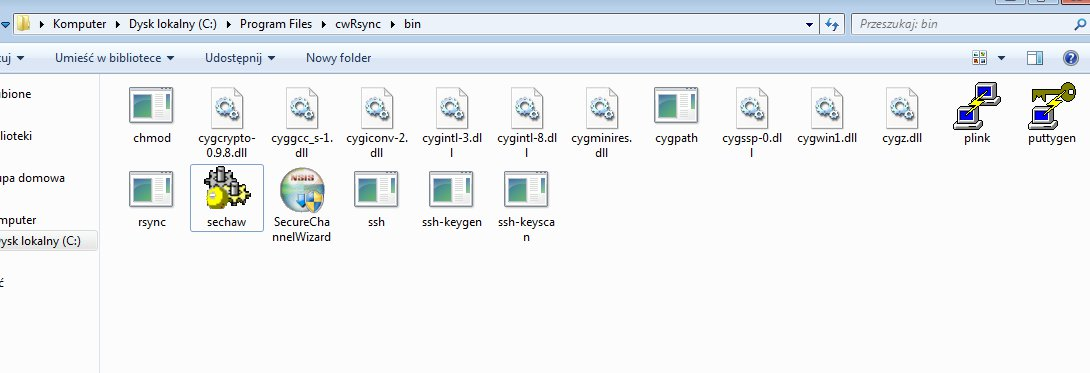
\includegraphics[width=1\textwidth]{img/i3.jpeg}
	\caption{Zawartość folderu ,,C:\textbackslash Program Files\textbackslash cwRsync\textbackslash bin''}
	\label{bin}
\end{figure}

\subsection{Instalacja Cygwin'a}
\label{full}
Alternatywą dla pomniejszonej wersji Cygwina (a dokładniej - bibliotek ,,.dll'' obsługujących Linuxowe API), jest jego pełna wersja. Polecam ją osobom, które chciałyby mieć choć część funkcjonalności Linuxowej na Windowsie. Z dostępnych programów mogę wymienić chociażby: ,,vim'', ,,apache'', ,,tetex'', ,,octave'', ,,cron'' i wiele innych.  Opis ten dedykowany także dla osób, które już posiadają ten program zainstalowany, a chcą uzupełnić go o opcję synchronizacji. \\
Proces instalacji przedstawię w kilku prostych krokach:
\begin{enumerate}
\item pobieramy najnowszą wersję Cygwin'a ze strony \verb|http://www.cygwin.com/setup.exe|
\item podczas instalacji wybieramy kolejno (po każdym klikając \verb|dalej|):
  \begin{itemize}
  \item ,,Install from Internet''
  \item podajemy katalog do instalacji, np. \verb|C:\cygwin|
  \item podajemy miejsce, gdzie mają trafiać ściągane pliki, np. \verb|C:\cyg_install|; po instalacji, można je usunąć
  \item jeśli łączymy się przez proxy, ustawiamy je w tym kroku, w przeciwnym wypadku - ,,Direct Connection''
  \item jako stronę, z której będą pobierane dane, możemy wybrać dowolną (wracamy i wybieramy inną, gdyby któraś z nich nie działała)
  \item w tym kroku rozwijamy listę ,,Net'' i wybieramy z niej ,,rsync'' - klikamy na \verb|Skip|, aż pojawi się najnowsza wersja (patrz rys. \ref{cyg_inst}); można tu skorzystać także z wyszukiwarki
  \item jeżeli chcemy korzystać z szyfrowanego połączenia poprzez SSH, wybieramy pakiet \verb|openssh|, także z listy ,,Net''
  \item na zakończenie instalacji możemy ustawić sobie skróty na pulpicie i/lub w Menu Start
  \end{itemize}
\end{enumerate}
W katalogu \verb|C:\cygwin\bin| pojawia nam się pożądana aplikacja \verb|rsync.exe|.
\begin{figure}[h!]
	\centering
	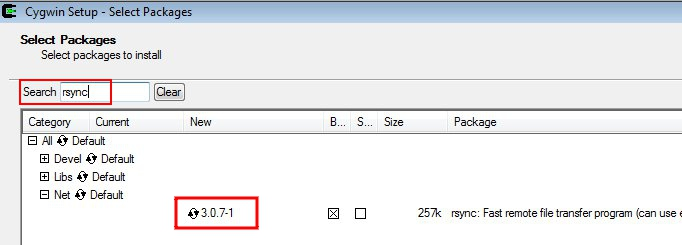
\includegraphics[width=0.8\textwidth]{img/i4.jpeg}
	\caption{Instalacja rsync w Cygwin'ie}
	\label{cyg_inst}
\end{figure}

\subsection{Skrypty}
\label{skrypty}
Tworzenie skryptów sprowadza się do uruchomienia dowolnego edytora tekstowego na systemie z rodziny Windows, np. Notatnika. Wystarczy skopiować jeden z moich skryptów, wkleić w edytorze i zapisać z rozszerzeniem ,,.bat'', np. ,,synchronizacja.bat''. Poniżej znajduje się ich lista podzielonych, w zależności od przeznaczenia i rodzaju synchronizacji, plików wsadowych. Jednak, przed przystąpieniem do ich uruchomienia, należy skonfigurować odpowiednie zmienne.
\subsubsection{Wersja pełna/minimalna Cygwina}
\label{pelmin}
W zależności od wybranej wersji, czy to pełnej (rozdział \ref{full}), czy też minimalnej (rozdział \ref{mini}), ustawiamy odpowiednio zmienną:
\begin{verbatim}
SET SCIEZKA=...
\end{verbatim}
Jako, że wersja pełna instaluje się standardowo w katalogu \verb|C:\cygwin|, dla tej wersji ustawiamy: \verb|SET SCIEZKA=C:\cygwin|. Dla wersji minimalnej, gdzie ścieżką domyślną jest \verb|C:\Program Files\cwRsync|, wpisujemy: \verb|SET SCIEZKA=%PROGRAMFILES%\cwRsync|\footnote{\%PROGRAMFILES\% to zmienna systemowa zawierającą lokalizację folderu ,,Program Files''}.

\subsubsection{Synchronizacja lokalna}
Poniżej listing pliku, który umożliwi synchronizację folderów lokalnych lub na zdalnym serwerze:
\begin{verbatim}
@echo off
cls
setlocal

SET PARAMETRY=avu
SET SCIEZKA=C:\cygwin
SET PATH=%SCIEZKA%\bin;%PATH%

rsync -%PARAMETRY% /cygdrive/c/katalog/ /cygdrive/d/inny_katalog
\end{verbatim}
\noindent
Jeżeli chcemy, dodajemy deklarację zmiennych:
\begin{verbatim}
SET CEL=/cygdrive/d/inny_katalog
SET ZRODLO=/cygdrive/c/katalog/
\end{verbatim}
Mamy wtedy: \fbox{rsync -\%PARAMETRY\% \%ZRODLO\% \%CEL\%}, dzięki czemu wygląda to przejrzyściej, a my sami ustawiamy jedynie zmienne, nie martwiąc się o składnię polecenia.\\

\noindent
Krótkie wyjaśnienie poszczególnych instrukcji:\\
\verb|@echo off, cls, setlocal| - wyłącza ciągłe wypisywanie ścieżki, czyści ekran i włącza możliwość definiowania zmiennych lokalnych, z których to będziemy korzystać,\\
\verb|SET PARAMETRY=...| - parametry synchronizacji,\\
\verb|SET SCIEZKA=...| - ścieżka, gdzie zainstalowano Cygwina (patrz \ref{pelmin}),\\
\verb|SET PATH=%SCIEZKA%\bin;%PATH%| - dopisywanie lokalizacji Cygwina do zmiennej systemowej, w której wyszukiwane są programy, dzięki czemu możemy użyć samej nazwy \verb|rsync|,\\
\verb|SET CEL=...| - podajemy miejsce docelowe,\\
\verb|SET ZRODLO=...| - podajemy lokalizację źródłową; tutaj wymagane jest dłuższe wyjaśnienie.\\W Windowsie ścieżki składają się z litery dysku (np. C, D, E), dwukropka i odwróconego ukośnika (np. \verb|C:\katalog|). Użycie znaku dwukropka, w składni polecenia \verb|rsync|, zostałoby potraktowane jako ścieżka do katalogu zdalnego, dlatego stosujemy tu konwencję znaną z UNIX'a, to jest: zamieniamy odwrócone ukośniki na nieodwrócone, a w miejsce litery dysku wpisujemy \verb|/cygdrive/<litera_dysku>|. W ten sposób nasza przykładowa lokalizacja wygląda następująco: \verb|/cygdrive/c/katalog|.\\

\subsubsection{Synchronizacja zdalna}
Dla synchronizacji zdalnej nie trzeba zbytnio zmieniać powyższego skryptu - wystarczy modyfikacja jednej zmiennej. Przy wysyłaniu na zdalny serwer, jako cel podajemy \verb|[LOGIN@]HOST:CEL|, na przykład: \\\verb|SET cel=spychalm@192.168.100.5:/home/spychalm/testowy|. \\
Pobieranie jest analogiczne - ustawiamy, jako źródło, \verb|[LOGIN@]HOST:ŹRÓDŁO|.
\\ Nie będę tutaj omawiać szczegółów, ponieważ wyjaśniłem wszystko w rozdziale \ref{zdaln}. 
\\\\
Przykład pobierania danych:
\begin{verbatim}
@echo off
cls
setlocal

SET ZRODLO=~/www/
SET CEL=/cygdrive/c/strona_www
SET PARAMETRY=av
SET SCIEZKA=C:\cygwin
SET PATH=%SCIEZKA%\bin;%PATH%

rsync -%PARAMETRY% spychalm@volt.iem.pw.edu.pl:%ZRODLO% %CEL%
\end{verbatim}

\subsubsection{Poprzez usługę rsyncd}
Podobnie jak poprzednio, skorzystamy z wcześniejszego opisu składni polecenia \verb|rsync|, wracając do rozdziału \ref{demon}. Można ustawić tu zmienne zgodnie ze schematem, jak przy synchronizacji zdalnej, jednak pokażę inne rozwiązanie. Zmienimy składnię polecenia \verb|rsync -%PARAMETRY% %ZRODLO% %CEL%|. \\
Dla wysyłania:\\\fbox{rsync -\%parametry\% \%zrodlo\% [LOGIN@]HOST::MODUL} \\lub\\ \fbox{rsync -\%parametry\% \%zrodlo\% rsync://[LOGIN@]HOST[:PORT]/\%cel\%} podając oczywiście login, host i moduł lub port i cel, do którego się odwołujemy.\\
Dla odbierania postępujemy analogicznie. Jedną z modyfikacji może być tu: \verb|rsync -%parametry% 192.168.100.5::wazne_dane /cygdrive/c/pobrane|.

\subsubsection{Za pomocą SSH}
Zastosować można tu co najmniej dwa rozwiązania: do parametrów dopisujemy \verb|e "ssh [-l <uzytkownik>] [-p <port>] ..."| lub to samo umieszczamy po \verb|rsync -%parametry%|. Przykład: \verb|set PARAMETRY=ave "ssh -l spychalm"|. Cały skrypt mógłby wyglądać następująco:
\begin{verbatim}
@echo off
cls
setlocal

SET LOGIN=spychalm
SET PORT=4321
SET HOST=edi.iem.pw.edu.pl
SET ZRODLO=/cygdrive/c/strona_www/
SET CEL=~/www
SET PARAMETRY=auve "ssh -l %LOGIN% -p %PORT%"
SET SCIEZKA=%PROGRAMFILES%\cwRsync
SET PATH=%SCIEZKA%\bin;%PATH%

rsync -%PARAMETRY% %ZRODLO% %HOST%:%CEL%
\end{verbatim}

\subsubsection{Podsumowanie}
Do każdego ze skryptów można dopisać na końcu linijkę \verb|PAUSE| - umożliwi ona wyświetlenie wyniku operacji - nie zamknie okna, jeśli wywołaliśmy skrypt bezpośrednio (to znaczy klikając na niego - nie z poziomu konsoli). W przypadku używania tych plików wsadowych w połączeniu z ,,Harmonogramem Zadań'', autostartem - kiedy jest automatycznie startowany, lepiej pominąć tą opcję (a nawet parametr \verb|verbose (-v)|), ponieważ w takiej sytuacji nie potrzebujemy okna z informacją. 

Oczywiście każdy może napisać od nowa lub dowolnie edytować te skrypty, stąd zamysł podania przeze mnie składni w rozdziale \ref{rsyncskladnia}. Celowo, za każdym razem, zmieniałem dane i parametry dla pokazania, że są one jedynie przykładem i każdy ustala je według własnych upodobań.

\subsection{Ustawianie kluczy w SSH}
Łącząc się ze zdalnym hostem poprzez SSH, jesteśmy za każdym razem pytani o hasło. Ciągłe jego wprowadzanie może okazać się niewygodne. Z pomocą przychodzi autoryzacja przy pomocy kluczy - dzięki czemu możemy ustawić zupełnie inne hasło lub nawet puste, czym zajmiemy się w tym rozdziale. Nie będę tu omawiał szczegółowo wszystkich parametrów komendy \verb|ssh-keygen|, ponieważ jest ona dokładnie opisana w internecie\cite{8}.
\\Całość sprowadza się do wykonania kilku kroków (działa tylko z pełną wersją Cygwina):
\begin{enumerate}
\item {\bf Uruchamiamy Cygwina}, z poziomu pulpitu (skrótu), lokalizacji programu (np. C:/cygwin/Cygwin.bat) lub Menu Start (Cygwin Bash Shell).
\item {\bf Generujemy klucze: publiczny i prywatny - \verb|$ssh-keygen -t rsa|}. Na pytanie o hasło/passphraze wciskamy enter. Polecenie wygeneruje dwa pliki, domyślnie w katalogu domowym w ,,ssh''. Pierwszy o nazwie ,,id\_rsa'' zawiera klucz prywatny, który nie może być nikomu udostępniany. Drugi o nazwie ,,id\_rsa.pub'' zawiera klucz publiczny, który wysyłamy na dowolny serwer, z którym zamierzamy ustanawiać połączenie.

\item {\bf Wysyłamy klucz publiczny na serwer}, z którym chcemy łączyć się bez hasła. Użyjemy do tego polecenia\footnote{można użyć tu innego sposobu wysyłania, jednak ten jest najprostszy} \verb|scp ~/ssh/id_rsa.pub [uzytkownik]@host:~/|

\item {\bf Logujemy się na zdalny host}, jeszcze przy pomocy hasła. Tam poleceniem \verb|cat ~/id_rsa.pub >> ~/ssh/authorized_keys|\footnote{jeżeli katalog ,,ssh'' nie istnieje, zakładamy go przy pomocy ,,mkdir ssh''} dodajemy nasz klucz do listy kluczy autoryzowanych do łączenia się z naszym hostem.
\end{enumerate}
Od tej pory mamy możliwość logowania się bez hasła do zdalnego serwera, a tym samym nasza zautomatyzowana synchronizacja nie będzie nas za każdym razem pytała o hasło, oczywiście zachowując bezpieczny kanał transmisji plików.

Dużym ułatwieniem jest skorzystanie z gotowego programu ,,ssh-copy-id''\cite{9}, który wykonuje wysyłanie i dopisanie klucza na zdalnym komputerze za nas. Generujemy klucze, a następnie uruchamiamy \verb|ssh-copy-id [uzytkownik]@host|.

\section{Testowanie}
Cały proces instalacji i konfiguracji przeprowadziłem początkowo na maszynie wirtualnej z zainstalowanym systemem Windows 7. Następnie całość powtórzyłem na innej maszynie wirtualnej z Windowsem XP oraz na komputerach, z zainstalowanymi tymi wersjami Windowsa, jako ich macierzystymi systemami operacyjnymi. Przykładowe programy (z rozdziału \ref{dosynch}.) testowane były tylko na systemach wirtualnych, z racji braku Windowsa na moim notebooku. Na żadnym z tych urządzeń nie zauważyłem problemu z pobieraniem, instalacją czy konfiguracją \verb|cwRsync|'a. Jednakże, może się tak zdarzyć, że podane przeze mnie strony internetowe lub wersje programów, nie będą dostępne. Należy wówczas skorzystać z wyszukiwarki internetowej i za jej pomocą znaleźć serwery lustrzane lub strony, gdzie podane oprogramowanie będzie możliwe do pobrania. 

\section{Wnioski}
Z synchronizacją danych spotykamy się na co dzień. Większość z nas kopiuje dane z jednego nośnika na inny - jedni robią to ,,ręcznie'', inni mają do tego skrypty. Osobiście uważam, że druga opcja jest znacznie korzystniejsza, zwłaszcza, gdy chcemy, by ten proces wykonywał się automatycznie. 

Pomimo dostępności mnogiej liczby programów do tego celu oraz przetestowania przeze mnie części z nich, stwierdzam, że żaden nie zastąpił szybkiego i łatwego rozwiązania konsolowego, a mianowicie programu \verb|rsync|. Po poświęceniu chwili czasu, mamy napisane różnorakie pliki wsadowe, do użycia, w zależności od potrzeb. Możemy je umieszczać na serwerach czy terminalach, nawet tych bez środowiska graficznego i uruchamiać je zdalnie. W systemach z rodziny Windows, dodając go do ,,Harmonogramu Zadań'', a w Linuxie - do zadań \verb|cron|'a, nie musimy ciągle pamiętać o zrobieniu kopii zapasowej. Uważam to za ogromne ułatwienie zwłaszcza dla osób, które mają z tym problemy. 




